
\documentclass[border=10pt, 12pt]{standalone}
\usepackage[svgnames]{xcolor}
\usepackage{amsmath}
\usepackage{pgfplots}
\pgfplotsset{compat=newest}
\usepackage[sfdefault]{FiraSans}
\usepackage{FiraMono}
\renewcommand*\familydefault{\sfdefault}
\begin{document}
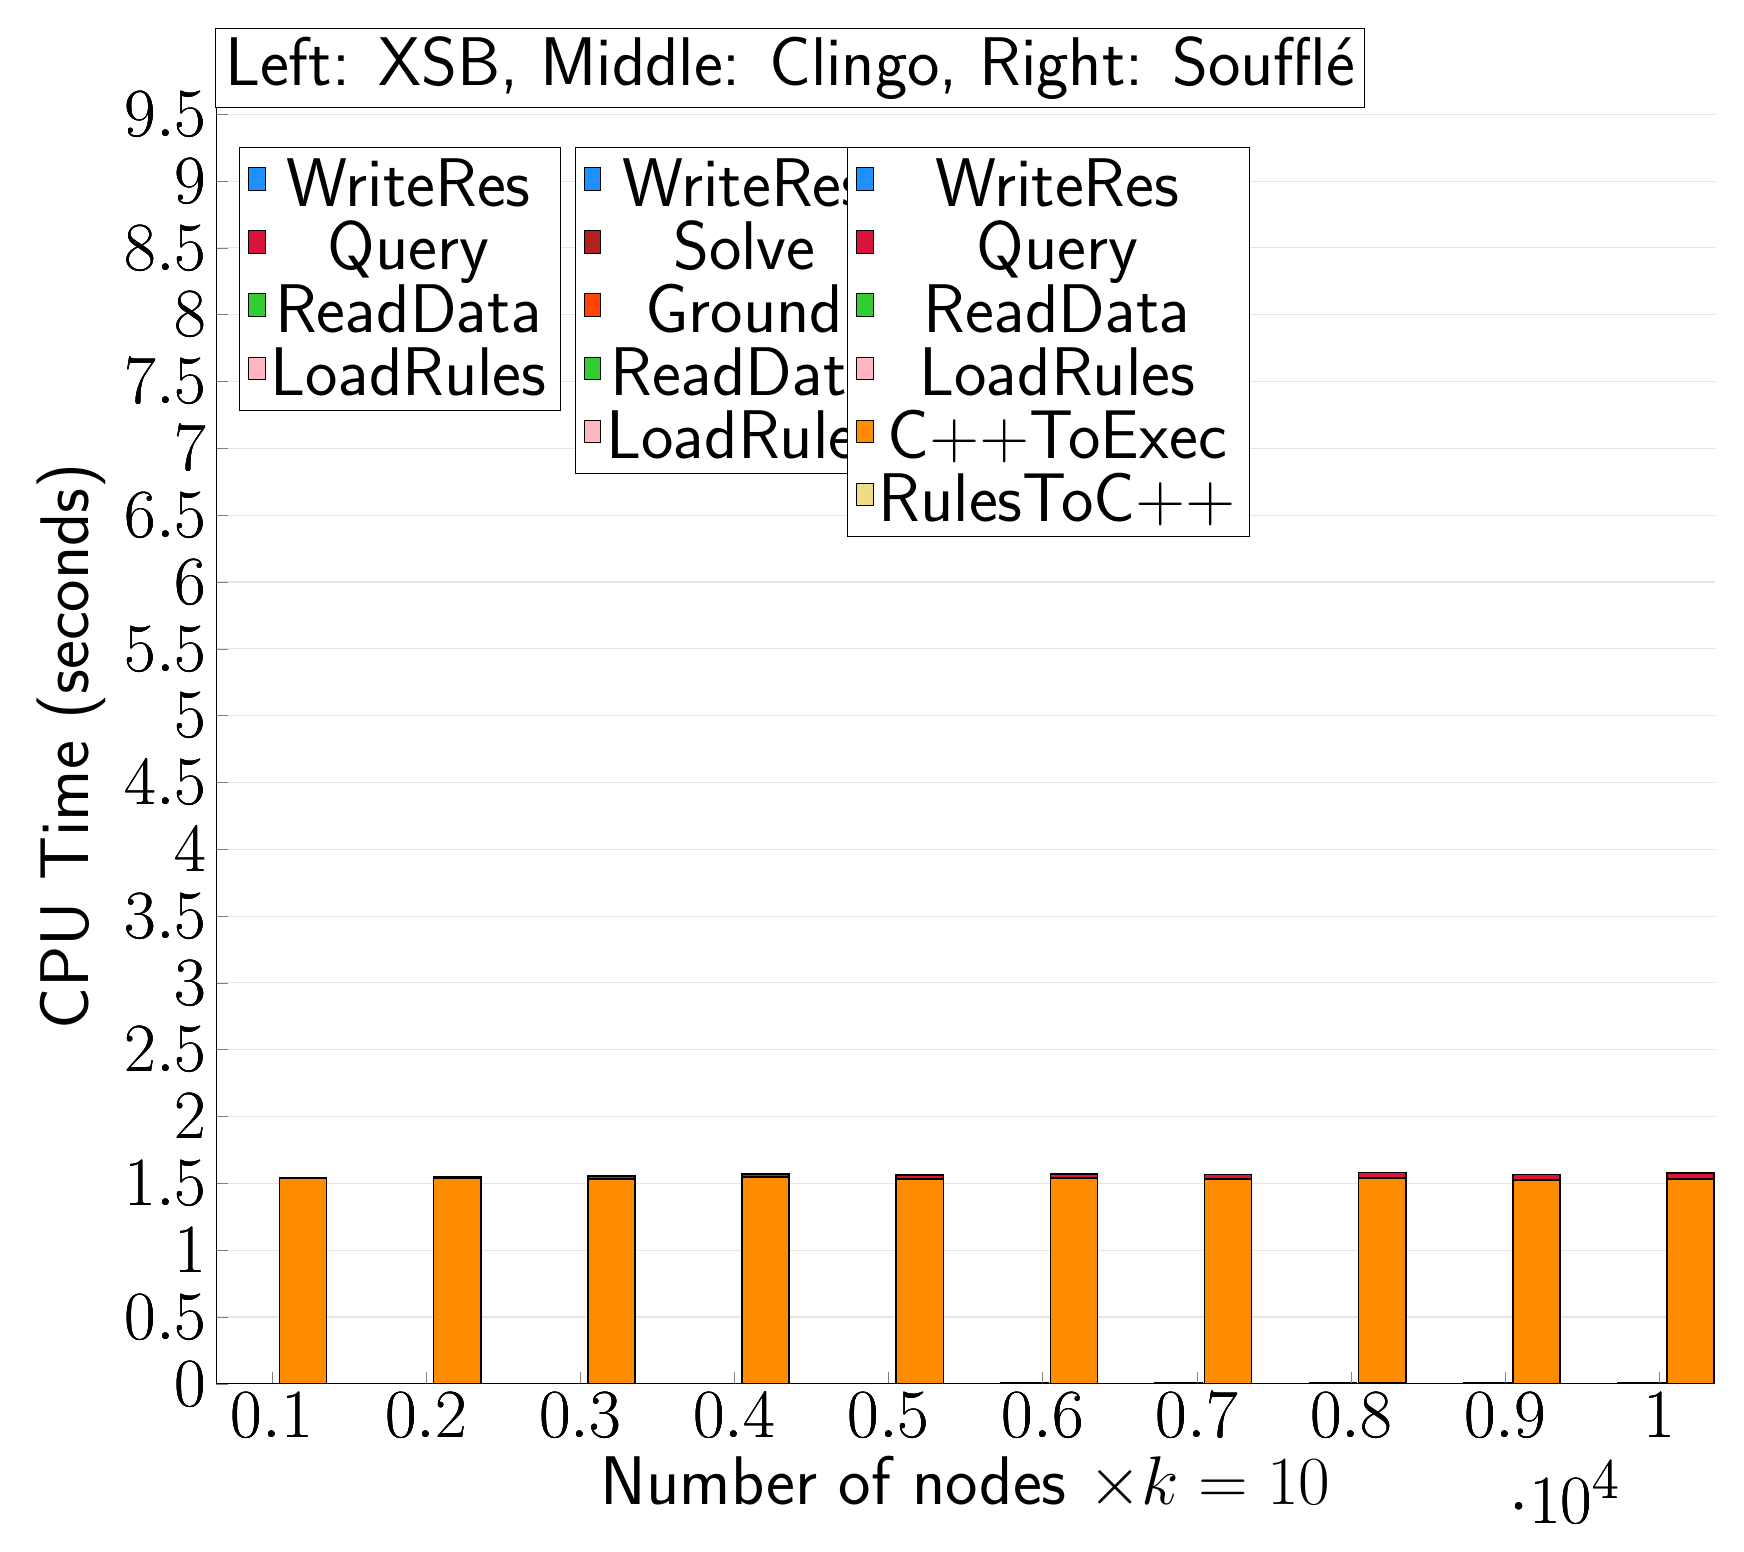
\begin{tikzpicture}
                        \begin{axis}[bar shift=-24.3pt, 
   ybar stacked,
   width=1.7\textwidth,
   bar width=0.6cm,
   ymajorgrids, tick align=inside,
   major grid style={draw=gray!20},
   xtick=data,
   ymin=0, ymax=9.544,
   axis x line*=bottom,
   axis y line*=left,
   enlarge x limits=0.04,
   legend style={
       at={(0.23, 0.97)},
       anchor=north east,
       legend columns=1,
       font=\Huge,
   },
   ylabel={CPU Time (seconds)},
   xlabel={Number of nodes $\times k=10$},
   label style={font=\Huge},
   tick label style={font=\Huge},
]
\addlegendimage{fill=DodgerBlue, draw=black, line width=0.2pt}
\addlegendentry{WriteRes}
\addlegendimage{fill=Crimson, draw=black, line width=0.2pt}
\addlegendentry{Query}
\addlegendimage{fill=LimeGreen, draw=black, line width=0.2pt}
\addlegendentry{ReadData}
\addlegendimage{fill=LightPink, draw=black, line width=0.2pt}
\addlegendentry{LoadRules}
\addplot +[fill=LightPink, draw=black, line width=0.55pt] coordinates {
(1000, 0.0005574000000000004)
(2000, 0.0005580000000000002)
(3000, 0.0005496)
(4000, 0.0005646000000000007)
(5000, 0.000555800000000001)
(6000, 0.0005528)
(7000, 0.0005558000000000006)
(8000, 0.0005507999999999994)
(9000, 0.0005570000000000007)
(10000, 0.0005553999999999991)
};
\addplot +[fill=LimeGreen, draw=black, line width=0.55pt] coordinates {
(1000, 0.0002057999999999996)
(2000, 0.0002871999999999994)
(3000, 0.0003608)
(4000, 0.00044299999999999955)
(5000, 0.0005161999999999999)
(6000, 0.0005923999999999995)
(7000, 0.0006825999999999996)
(8000, 0.0007516000000000005)
(9000, 0.0008319999999999994)
(10000, 0.0009308000000000007)
};
\addplot +[fill=Crimson, draw=black, line width=0.55pt] coordinates {
(1000, 2.0200000000000078e-05)
(2000, 2.080000000000034e-05)
(3000, 2.099999999999986e-05)
(4000, 2.0799999999999997e-05)
(5000, 2.0399999999999598e-05)
(6000, 2.060000000000048e-05)
(7000, 2.05999999999998e-05)
(8000, 2.10000000000002e-05)
(9000, 2.040000000000028e-05)
(10000, 2.099999999999952e-05)
};
\addplot +[fill=DodgerBlue, draw=black, line width=0.55pt] coordinates {
(1000, 6.419999999999966e-05)
(2000, 6.239999999999992e-05)
(3000, 6.38000000000003e-05)
(4000, 6.440000000000021e-05)
(5000, 6.460000000000039e-05)
(6000, 6.459999999999936e-05)
(7000, 6.76e-05)
(8000, 6.339999999999989e-05)
(9000, 6.479999999999956e-05)
(10000, 6.520000000000027e-05)
};
\end{axis}

\begin{axis}[bar shift=-6.5pt, 
   ybar stacked,
   width=1.7\textwidth,
   bar width=0.6cm,
   ymajorgrids, tick align=inside,
   major grid style={draw=none},
   xtick=data,
   ymin=0, ymax=9.544,
   axis x line*=none,
   axis y line*=none,
   enlarge x limits=0.04,
   legend style={
       at={(0.454, 0.97)},
       anchor=north east,
       legend columns=1,
       font=\Huge,
   },
   label style={font=\Huge},
   tick label style={font=\Huge},
]
\addlegendimage{fill=DodgerBlue, draw=black, line width=0.2pt}
\addlegendentry{WriteRes}
\addlegendimage{fill=FireBrick, draw=black, line width=0.2pt}
\addlegendentry{Solve}
\addlegendimage{fill=OrangeRed, draw=black, line width=0.2pt}
\addlegendentry{Ground}
\addlegendimage{fill=LimeGreen, draw=black, line width=0.2pt}
\addlegendentry{ReadData}
\addlegendimage{fill=LightPink, draw=black, line width=0.2pt}
\addlegendentry{LoadRules}
\addplot +[fill=LightPink, draw=black, line width=0.55pt] coordinates {
(1000, 0.0)
(2000, 0.0)
(3000, 0.0)
(4000, 0.0)
(5000, 0.0)
(6000, 0.0)
(7000, 0.0)
(8000, 0.0)
(9000, 0.0)
(10000, 0.0)
};
\addplot +[fill=LimeGreen, draw=black, line width=0.55pt] coordinates {
(1000, 0.0)
(2000, 0.0)
(3000, 0.0)
(4000, 0.0)
(5000, 0.0)
(6000, 0.0)
(7000, 0.0)
(8000, 0.0)
(9000, 0.0)
(10000, 0.0)
};
\addplot +[fill=OrangeRed, draw=black, line width=0.55pt] coordinates {
(1000, 0.0)
(2000, 0.0)
(3000, 0.0)
(4000, 0.0020000000000000018)
(5000, 0.0020000000000000018)
(6000, 0.008000000000000007)
(7000, 0.010000000000000009)
(8000, 0.010000000000000009)
(9000, 0.010000000000000009)
(10000, 0.010000000000000009)
};
\addplot +[fill=FireBrick, draw=black, line width=0.55pt] coordinates {
(1000, 0.0)
(2000, 0.0)
(3000, 0.0)
(4000, 0.0020000000000000018)
(5000, 0.0)
(6000, 0.0)
(7000, 0.0)
(8000, 0.0)
(9000, 0.0)
(10000, 0.0)
};
\addplot +[fill=DodgerBlue, draw=black, line width=0.55pt] coordinates {
(1000, 0.0)
(2000, 0.0)
(3000, 0.0)
(4000, -0.0020000000000000018)
(5000, 0.0)
(6000, 0.0)
(7000, 0.0)
(8000, 0.0)
(9000, 0.0)
(10000, 0.0)
};
\end{axis}

\begin{axis}[bar shift=11.3pt, 
   ybar stacked,
   width=1.7\textwidth,
   bar width=0.6cm,
   ymajorgrids, tick align=inside,
   major grid style={draw=none},
   xtick=data,
   ymin=0, ymax=9.544,
   axis x line*=none,
   axis y line*=none,
   enlarge x limits=0.04,
   legend style={
       at={(0.69, 0.97)},
       anchor=north east,
       legend columns=1,
       font=\Huge,
   },
   label style={font=\Huge},
   tick label style={font=\Huge},
]
\addlegendimage{fill=DodgerBlue, draw=black, line width=0.2pt}
\addlegendentry{WriteRes}
\addlegendimage{fill=Crimson, draw=black, line width=0.2pt}
\addlegendentry{Query}
\addlegendimage{fill=LimeGreen, draw=black, line width=0.2pt}
\addlegendentry{ReadData}
\addlegendimage{fill=LightPink, draw=black, line width=0.2pt}
\addlegendentry{LoadRules}
\addlegendimage{fill=DarkOrange, draw=black, line width=0.2pt}
\addlegendentry{C++ToExec}
\addlegendimage{fill=LightGoldenrod, draw=black, line width=0.2pt}
\addlegendentry{RulesToC++}
\addplot +[fill=LightGoldenrod, draw=black, line width=0.55pt] coordinates {
(1000, 0.0)
(2000, 0.0)
(3000, 0.0020000000000000005)
(4000, 0.0020000000000000005)
(5000, 0.0)
(6000, 0.004000000000000001)
(7000, 0.0020000000000000005)
(8000, 0.008000000000000002)
(9000, 0.0020000000000000005)
(10000, 0.004000000000000001)
};
\addplot +[fill=DarkOrange, draw=black, line width=0.55pt] coordinates {
(1000, 1.536)
(2000, 1.538)
(3000, 1.532)
(4000, 1.544)
(5000, 1.5340000000000003)
(6000, 1.5340000000000003)
(7000, 1.528)
(8000, 1.532)
(9000, 1.52)
(10000, 1.528)
};
\addplot +[fill=LightPink, draw=black, line width=0.55pt] coordinates {
(1000, 0.000161)
(2000, 0.00015900000000000002)
(3000, 0.0001594)
(4000, 0.0001634)
(5000, 0.00015999999999999999)
(6000, 0.0001552)
(7000, 0.0001572)
(8000, 0.0001666)
(9000, 0.00015979999999999998)
(10000, 0.00016620000000000003)
};
\addplot +[fill=LimeGreen, draw=black, line width=0.55pt] coordinates {
(1000, 0.000926)
(2000, 0.0011794)
(3000, 0.0016428000000000002)
(4000, 0.0018658000000000001)
(5000, 0.0024602)
(6000, 0.0025732000000000003)
(7000, 0.0030733999999999996)
(8000, 0.0035214)
(9000, 0.0036452)
(10000, 0.0041732)
};
\addplot +[fill=Crimson, draw=black, line width=0.55pt] coordinates {
(1000, 0.006661)
(2000, 0.0117512)
(3000, 0.0175158)
(4000, 0.020787800000000002)
(5000, 0.0258136)
(6000, 0.029349999999999998)
(7000, 0.0335586)
(8000, 0.0364872)
(9000, 0.040042999999999995)
(10000, 0.0410854)
};
\addplot +[fill=DodgerBlue, draw=black, line width=0.55pt] coordinates {
(1000, 0.00037559999999999997)
(2000, 0.00026720000000000004)
(3000, 0.0002654)
(4000, 0.0002534)
(5000, 0.0002734)
(6000, 0.00023960000000000002)
(7000, 0.00023699999999999996)
(8000, 0.00023840000000000002)
(9000, 0.00024200000000000003)
(10000, 0.0002516)
};
\end{axis}


\node[anchor=south, draw, fill=white] at (rel axis cs:0.42,1) {\Huge Left: XSB, Middle: Clingo, Right: Soufflé};
\end{tikzpicture}
\end{document}
                    